\chapter{Introduction}
This is one of the most important components of the dissertation. It should begin with a clear statement of what the project is about so that the nature and scope of the project can be understood by a lay reader. It should summarise everything you set out to achieve, provide a clear summary of the project's background and relevance to other work and give pointers to the remaining sections of the dissertation which contain the bulk of the technical material.

Further information can be found here: \url{https://goo.gl/k2huN9}.

\section{\LaTeX{} code examples and formatting tips}
Hello, here's a citation \cite{greenwade93}. References are stored in a Bibtex file. Google Scholar and IEEExplore allow you to download citations of papers in Bibtex format from their search engine. Some people use JabRef (\url{http://www.jabref.org}) to manage their database of references.

This is an inline equation $\Gamma(t)=K_i e^{\sin^2(\omega_t)}$. The first paragraph appears without indent but the following ones will have an indentation.

This is an actual named equation:
\begin{equation}
v(x)=\frac{1}{2}\sin(2 \omega t + \phi) e^{-j s t}
\label{eq:cacona}
\end{equation}
\noindent where $\omega$ is the angular speed. Notice that symbols liks $\omega$ should be written in italics whereas measurement units such as V for Volts appear as normal text. This paragraph didn't have an indentation because the first sentence was linked to the definition of equation (\ref{eq:cacona}). A code snippet for an example program is shown in Listing~\ref{lst:code1}.

\begin{lstlisting}[caption=Source code for {\it hello.m},label=lst:code1,breaklines=true,basewidth=4pt,prebreak=**,postbreak=**,frame=single]
for i:=maxint to 0 do
begin
{ do nothing }
end;
Write('Case insensitive ');
Write('Pascal keywords.');
\end{lstlisting}

The characteristic parameters of the system are sumarised in Table~\ref{tab:tab1}. A figure is shown Fig~\ref{fig:felix}, we don't necessarily know if this figure will appear below, above or elsewhere; therefore, the text should never refer to the figure with sentences such as {\it "As shown here:"}.

\begin{figure}[htbp]
\centering

\includegraphics[width=0.3\linewidth]{introduction/fig/Felix_the_cat.pdf}
\caption{Felix the Cat}
\label{fig:felix}
\end{figure}

\begin{table}[htbp]
	\centering
	\begin{tabular}{lll}
		Parameter & Value & Units\\
		\hline
		$P$ & 1 & kW \\
		$Q$ & 0 & kVAr\\
	    \hline
	\end{tabular}
	\caption{Characteristic parameters of the system}
	\label{tab:tab1}
\end{table}

\begin{samepage}
Sometimes, the symbols in an equation are defined as follows\footnote{Some authors like to define their symbols this way.}:
\begin{equation}
	V(t)=A \sin(\omega t+\theta_0)
\end{equation}
\begin{tabular}{lll}
	where & $V$ & is a voltage waveform,\\
	& $A$ & is the amplitude of the voltage,\\
	& $\omega$ & is the angular frequency,\\
	& $t$ & is the time.
\end{tabular}
\end{samepage}

\subsection{A brief comparison between a proper plot and a horrible plot}

Figure \ref{fig:fig2} contains two plots of the same waveform. Subfigure \ref{fig:fig2sub1} shows a badly formatted figure, Subfigure \ref{fig:fig2sub2} shows a much better formatted figure. The problems with Subfigure \ref{fig:fig2sub1}, listed by order or relevance, are the following:

\begin{enumerate}
    \item The font size is too small to be read properly.
    \item The axes aren't labeled properly: the horizontal axis is not labeled and the units of the vertical axis are unknown. Further, symbols must be written in italics whereas numbers and units must be written as normal text.
    \item The choice of limits for the axes is not good, the figure has wide useless empty spaces. The most relevant part of the waveform is the transient that happens between times $t=$0 and $t=$0.05 s, which is less than 10\% of the timespan shown in the figure.
    \item The figure has been scaled without keeping the original aspect ratio and fonts look narrower than they would if the figure had been scaled properly.
    \item The plot doesn't have grid lines. This makes it hard to read the exact value (ie time, voltage) of points in the trace.
    \item The width of the trace is too thin and may not be visible if printed in low resolution.
    \item The choice of units of the vertical axis aren't the best. For example, in this case the plot would be easier to read if voltage had been expressed in kV instead of V.
    \item The figure was exported as a bitmap (e.g. png, jpg, bmp) instead of being exported in vector format (e.g. eps, svg, pdf) and visual artifacts appear when the figure is scaled up or down in order to fit in the document.
\end{enumerate}

\begin{figure}[htbp]
	\centering
	\subfigure[A horrible one.]{
		\label{fig:fig2sub1}
        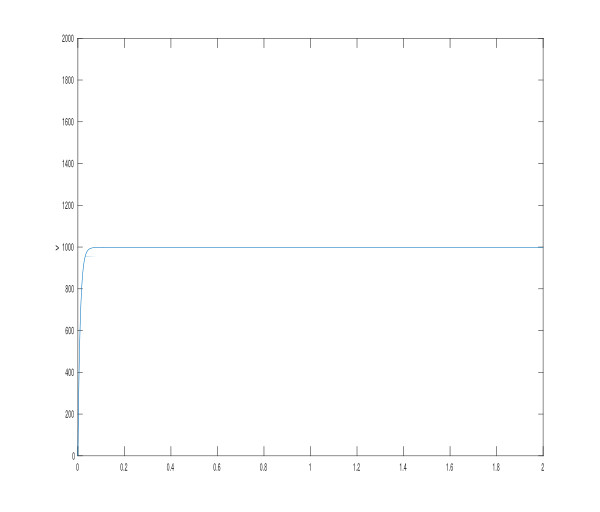
\includegraphics[width=0.5\linewidth]{introduction/fig/figure1.jpg}}
	\subfigure[A proper one.]{
		\label{fig:fig2sub2}
		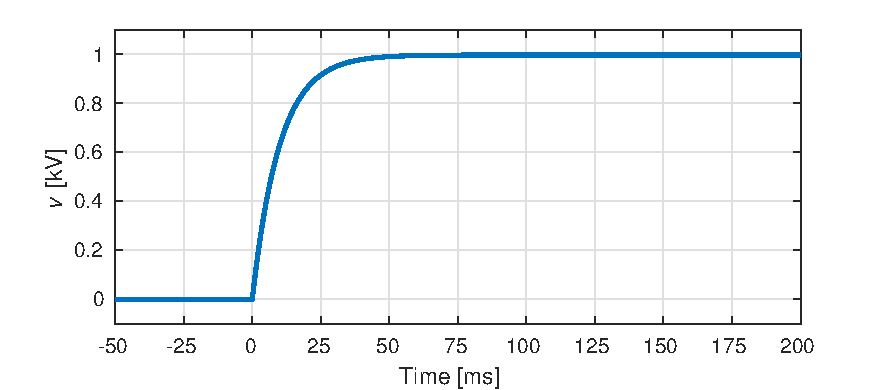
\includegraphics[width=0.6\linewidth]{introduction/fig/figure2.pdf}}
	\caption{A figure with two subfigures.}
	\label{fig:fig2}
\end{figure}

\begin{landscape}
	\begin{figure}[htbp]
\centering

\includegraphics[width=0.5\linewidth]{introduction/fig/Felix_the_cat.pdf}
\caption{Here's a large drawing of Felix the Cat that wouldn't fit in a portrait page}
\label{fig:felix2}
\end{figure}
\end{landscape}

\section{Objectives}
\section{Challenges}
\section{Contributions}